\documentclass[t]{beamer}
\usepackage[T1]{fontenc}
\usepackage[utf8]{inputenc}
\usepackage{lmodern}
\usepackage{lmodern}
\usepackage{biblatex} 
\usepackage{amsmath}
\usepackage{amsfonts}
\usepackage{amssymb}
\usepackage{amsthm}
\usepackage{graphicx}
\usepackage{color}
\usepackage{xcolor}
\usepackage{url}
\usepackage{textcomp}
\usepackage{hyperref}
\usepackage{parskip}
\usepackage{svg}
\usepackage{caption}

\usetheme{CambridgeUS}
\AtBeginBibliography{\footnotesize}
\addbibresource{presentation.bib}

\makeatletter
\setbeamertemplate{footline}
{
  \leavevmode%
  \hbox{%
  \begin{beamercolorbox}[wd=.333333\paperwidth,ht=2.25ex,dp=1ex,center]{author in head/foot}%
    \usebeamerfont{author in head/foot}\insertshortauthor%~~\beamer@ifempty{\insertshortinstitute}{}{(\insertshortinstitute)}
  \end{beamercolorbox}%
  \begin{beamercolorbox}[wd=.333333\paperwidth,ht=2.25ex,dp=1ex,center]{title in head/foot}%
    \usebeamerfont{title in head/foot}\insertshorttitle
  \end{beamercolorbox}%
  \begin{beamercolorbox}[wd=.333333\paperwidth,ht=2.25ex,dp=1ex,right]{date in head/foot}%
    \usebeamerfont{date in head/foot}\insertshortdate{}\hspace*{2em}
    \insertframenumber{} / \inserttotalframenumber\hspace*{2ex} 
  \end{beamercolorbox}}%
  \vskip0pt%
}
\makeatother

\title{Knowledge-Based Question Answering}
\author{Sudipto Ghosh}
\institute{\emph{M.Sc. CS Semester I\\Department of Computer Science\\University of Delhi}}
\date{\today}

\begin{document}

\begin{frame}
    \titlepage
\end{frame}

\begin{frame}
    \frametitle{Overview}
    \tableofcontents
\end{frame}

\section{Initial Tasks}
\begin{frame}[c]
   \frametitle{Initial Tasks}
    
   \centering 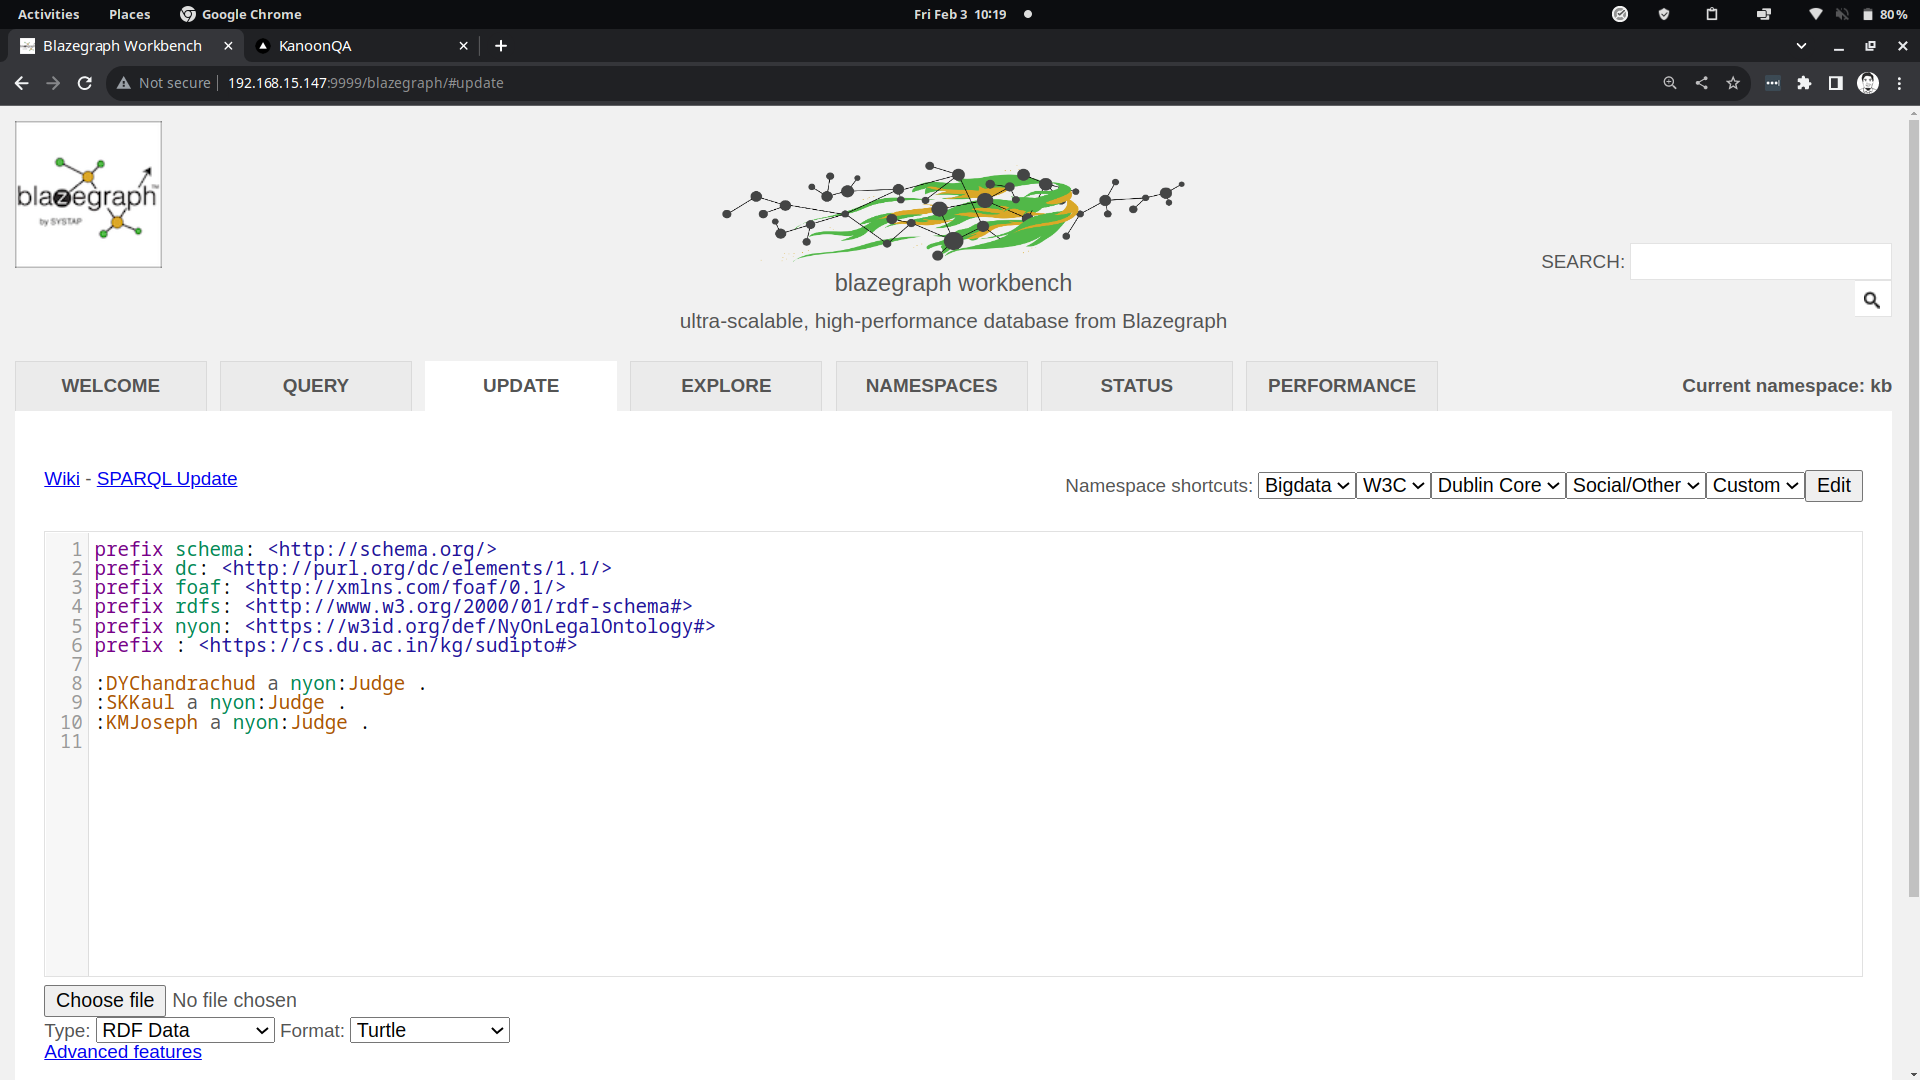
\includegraphics[width=340pt]{./Screenshot from 2023-02-03 10-19-32.png}
   
   \tiny{loading handpicked triples into triple store}
\end{frame}

\begin{frame}[c]
   \frametitle{Initial Tasks}
    
   \centering 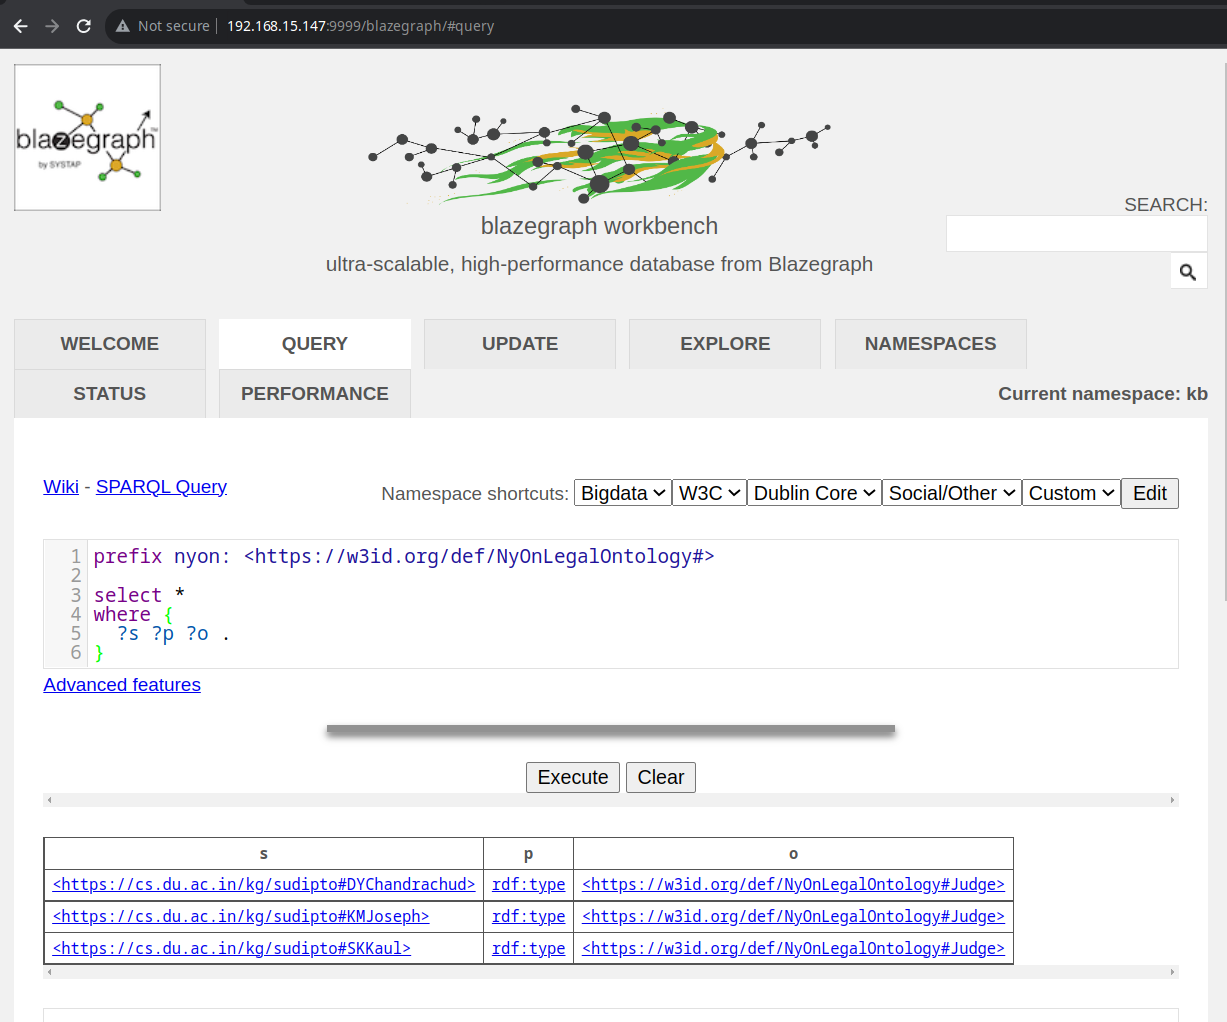
\includegraphics[width=225pt]{./Screenshot from 2023-02-03 10-32-08.png}
   
   \tiny{querying the triple store}
\end{frame}

\begin{frame}
    \frametitle{Initial Tasks}

    \centering 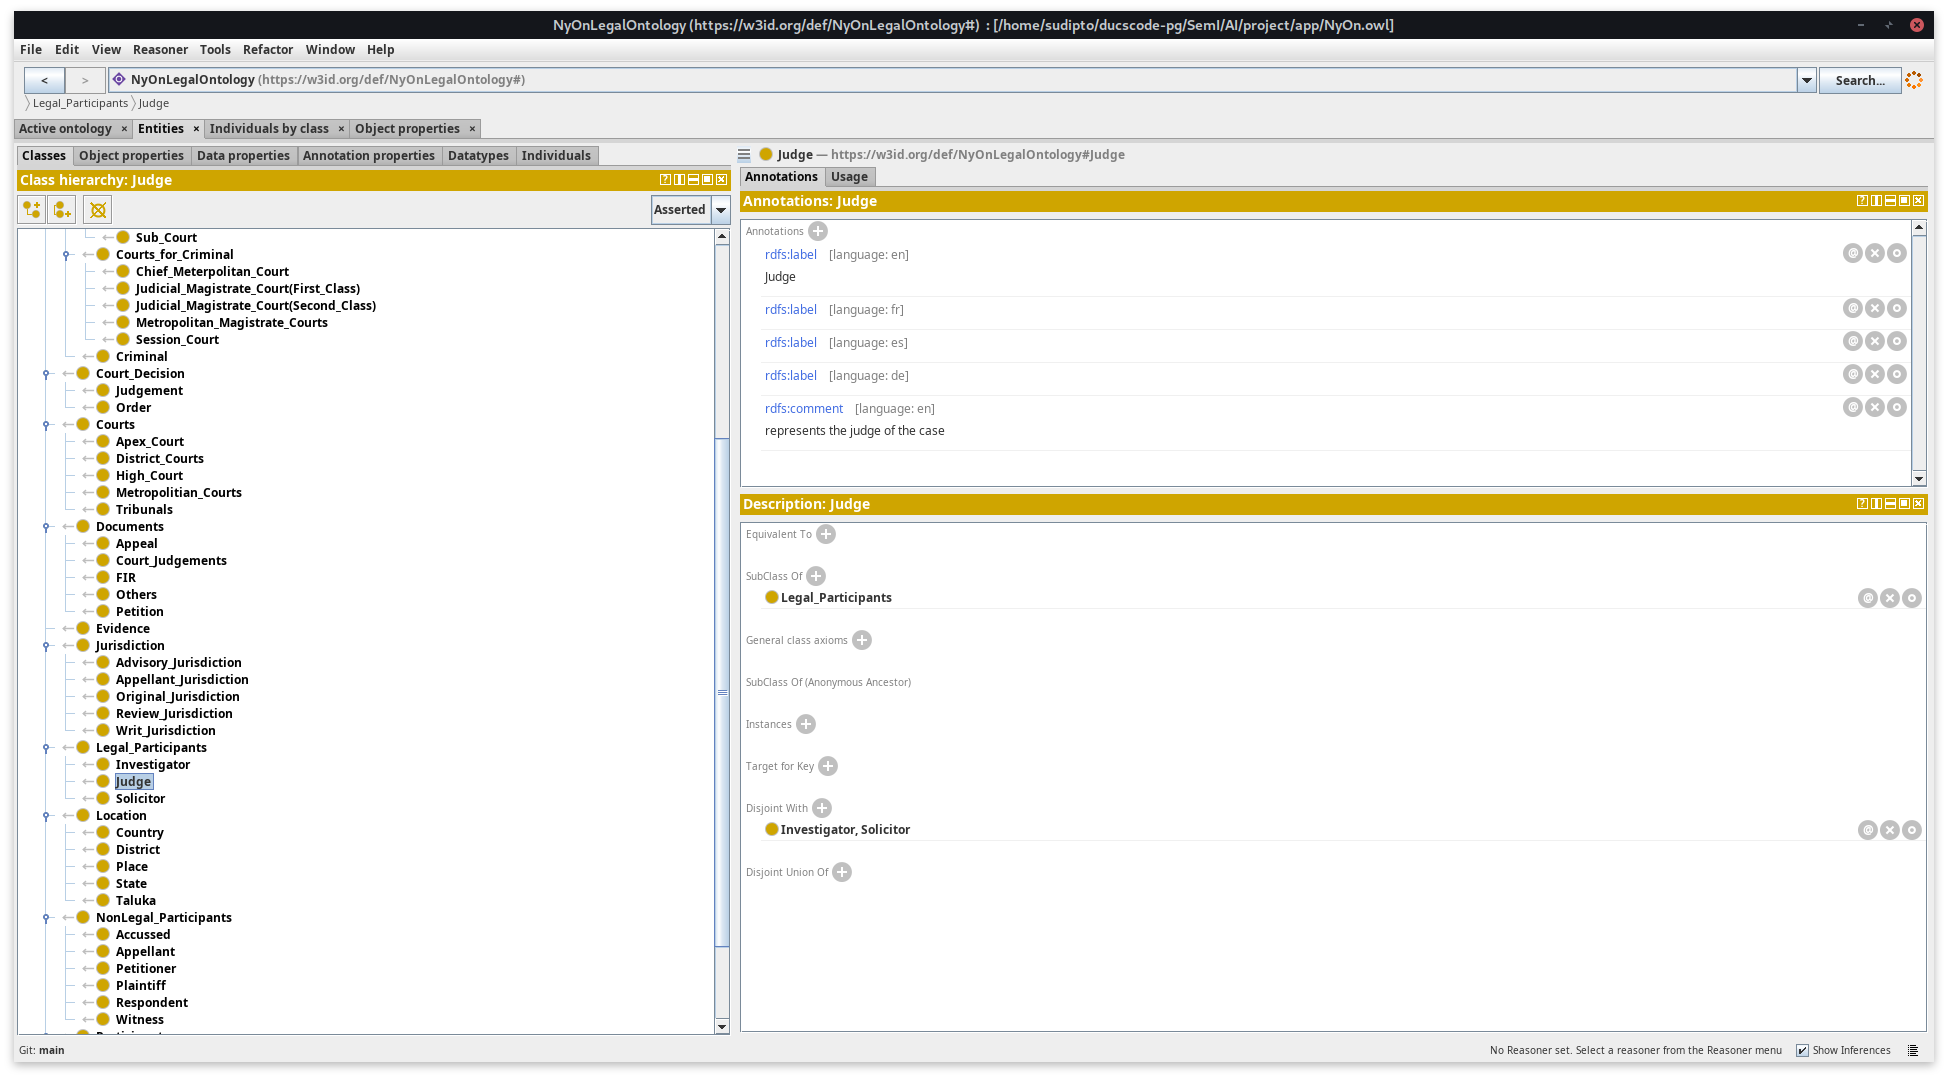
\includegraphics[width=320pt]{./Screenshot from 2023-02-03 10-43-34.png}
    
   \tiny{inspecting nyon ontology with protege}
\end{frame}

\begin{frame}
    \frametitle{Initial Tasks}

    \centering 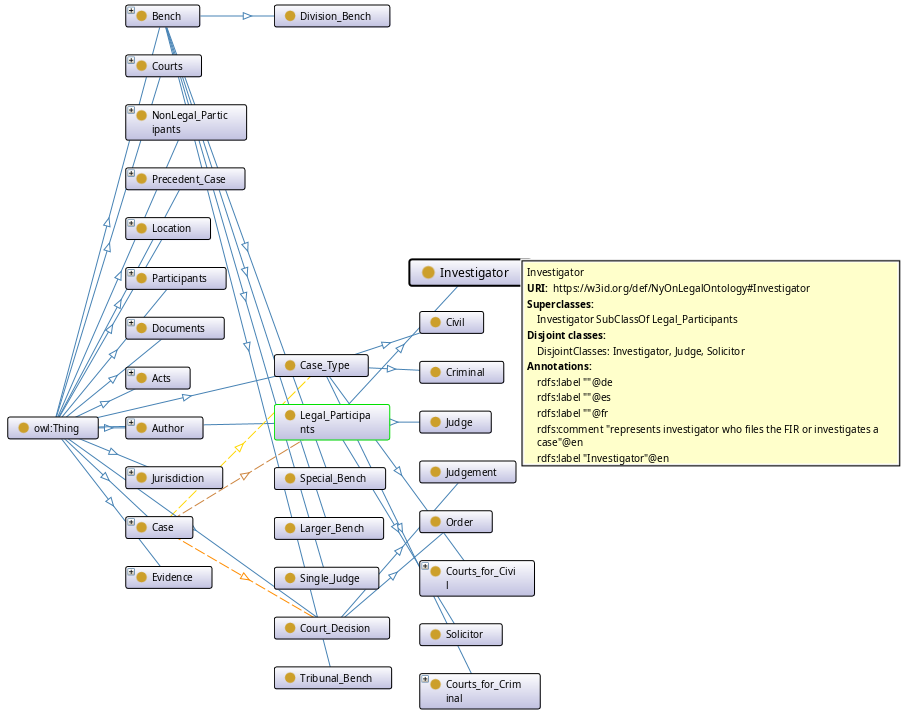
\includegraphics[width=320pt]{./Screenshot from 2023-02-03 10-50-31.png}
    
   \tiny{inspecting nyon ontology with protege}
\end{frame}

\section{Basic Prototype}
\begin{frame}
    \frametitle{Basic Prototype}

    \centering 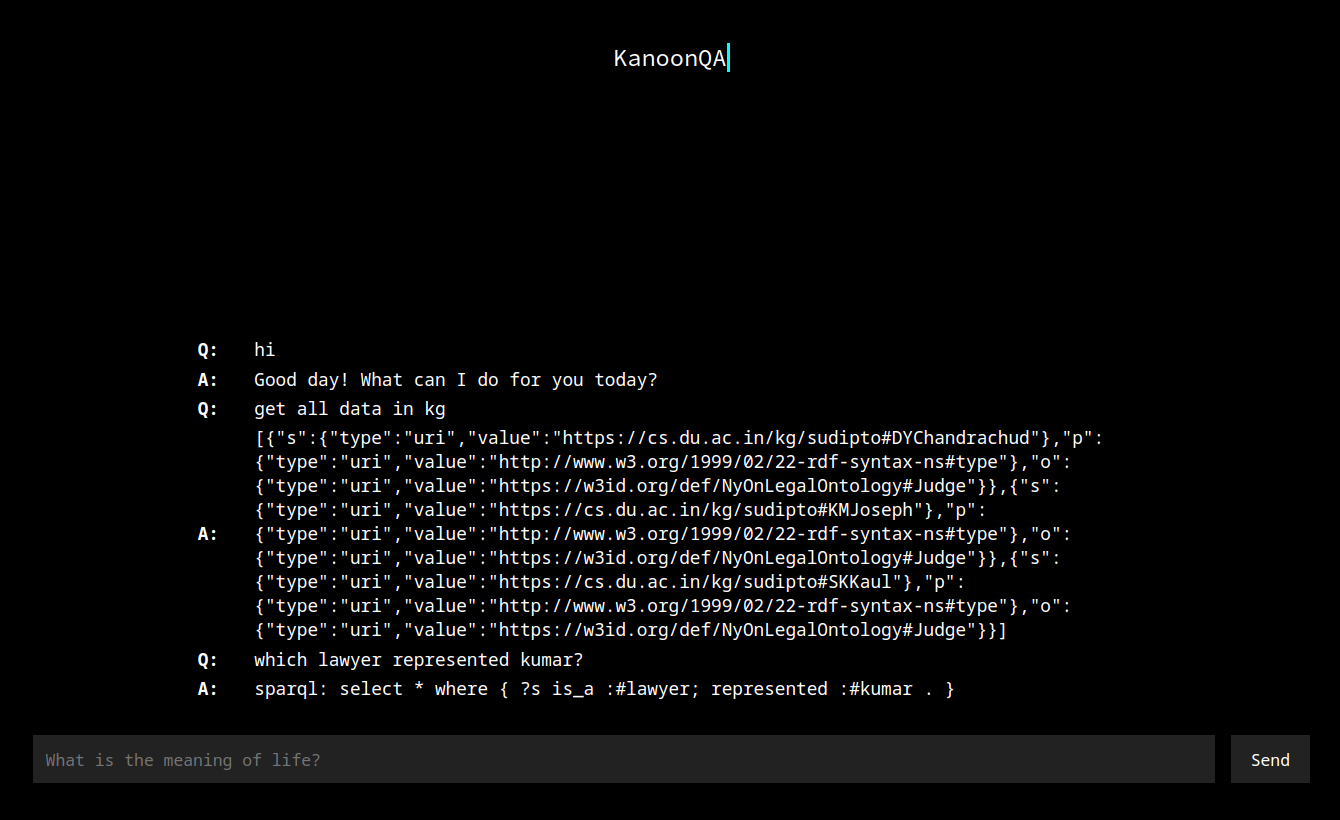
\includegraphics[width=300pt]{./Screenshot from 2023-02-03 10-34-36.png}\\
   \tiny{user interface and basic output\\tech stack: next.js, google cloud platform}
\end{frame}

\end{document}